% 直三棱柱ABC-A1B1C1侧视示意:顶/底/中三棱水平,CE竖直,E为AB中点;截面ACB1中CB1/AB1虚线
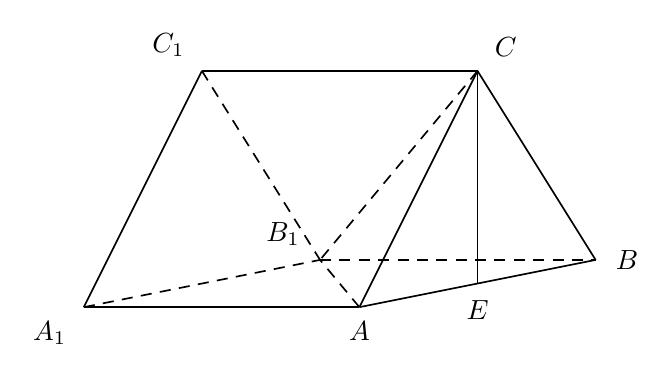
\begin{tikzpicture}[x=1cm,y=1cm,font=\normalsize,line width=.6pt,
  solid edge/.style={solid,line width=.6pt},
  hidden edge/.style={dashed,line width=.6pt,dash pattern=on 4pt off 3pt},
  geom label/.style={font=\normalsize,inner sep=2pt}]
\coordinate (A) at (3.0,0.0);
\coordinate (B) at (6.0,0.6);
\coordinate (E) at (4.5,0.3);
\coordinate (C) at (4.5,3.0);
\coordinate (A1) at (-0.5,0.0);
\coordinate (B1) at (2.5,0.6);
\coordinate (C1) at (1.0,3.0);
% lateral edges
\draw[solid edge] (A1) -- (A);
\draw[solid edge] (C1) -- (C);
\draw[hidden edge] (B1) -- (B);
% base ABC (front, all visible)
\draw[solid edge] (A) -- (B);
\draw[solid edge] (B) -- (C);
\draw[solid edge] (A) -- (C);
% base A1B1C1 (back, partly hidden)
\draw[solid edge] (A1) -- (C1);
\draw[hidden edge] (A1) -- (B1);
\draw[hidden edge] (C1) -- (B1);
% section ACB1
\draw[hidden edge] (A) -- (B1);
\draw[hidden edge] (C) -- (B1);
% segment CE
\draw[solid edge] (C) -- (E);
% labels with clearance
\node[geom label,below left] at ([xshift=-4pt,yshift=-3pt]A1) {$A_{1}$};
\node[geom label,below] at ([yshift=-3pt]A) {$A$};
\node[geom label,right] at ([xshift=5pt]B) {$B$};
\node[geom label,below] at ([yshift=-4pt]E) {$E$};
\node[geom label,above right] at ([xshift=4pt,yshift=3pt]C) {$C$};
\node[geom label,above left] at ([xshift=-4pt,yshift=3pt]C1) {$C_{1}$};
\node[geom label,above left] at ([xshift=-5pt,yshift=3pt]B1) {$B_{1}$};
\end{tikzpicture}
